% $Header: /home/vedranm/bitbucket/beamer/solutions/generic-talks/generic-ornate-15min-45min.en.tex,v 90e850259b8b 2007/01/28 20:48:30 tantau $

\documentclass[]{beamer}

% This file is a solution template for:

% - Giving a talk on some subject.
% - The talk is between 15min and 45min long.
% - Style is ornate.

%
% In principle, this file can be redistributed and/or modified under
% the terms of the GNU Public License, version 2.
%
% However, this file is supposed to be a template to be modified
% for your own needs. For this reason, if you use this file as a
% template and not specifically distribute it as part of a another
% package/program, I grant the extra permission to freely copy and
% modify this file as you see fit and even to delete this copyright
% notice. 


\mode<presentation>
{
  \usetheme{Spil}
  % or ...

  \setbeamercovered{transparent}
  % or whatever (possibly just delete it)
}

\usepackage[english]{babel}
\usepackage[latin1]{inputenc}

\usepackage{times}
\usepackage[T1]{fontenc}

\title[]{Testing in Erlang}
%\subtitle
%{Presentation Subtitle} % (optional)

\author[] % (optional, use only with lots of authors)
{Enrique Paz}

\institute[] % (optional, but mostly needed)
{Senior Backend Developer @ Team Services}

\date[] % (optional)
{EUGNL / 12-07-2012}


% If you have a file called "university-logo-filename.xxx", where xxx
% is a graphic format that can be processed by latex or pdflatex,
% resp., then you can add a logo as follows:

% \pgfdeclareimage[height=0.5cm]{university-logo}{university-logo-filename}
% \logo{\pgfuseimage{university-logo}}


% Delete this, if you do not want the table of contents to pop up at
% the beginning of each subsection:
\AtBeginSubsection[]
{
  \begin{frame}<beamer>{Outline}
    \tableofcontents[currentsection,currentsubsection]
  \end{frame}
}


% If you wish to uncover everything in a step-wise fashion, uncomment
% the following command: 
%\beamerdefaultoverlayspecification{<+->}

\begin{document}

\begin{frame}
  \titlepage
\end{frame}

\begin{frame}{Index}
  \tableofcontents
  % You might wish to add the option [pausesections]
\end{frame}

\section{Introduction}

\subsection*{Why should I test?}
\label{why_should_i_test}

\begin{frame}{Reasons for testing}
    \begin{itemize}
    \item It increases your confidence in the code you write
    \pause
    \item Tests themselves are useful documentation
    \pause
    \item It makes refactoring \emph{really} an option
    \pause
    \item It helps finding bugs earlier, so the impact is much lower
    \end{itemize}
\end{frame}

\begin{frame}{Yeah, but...}
    \begin{itemize}
    \item \textit{``My code is so clear/simple it doesn't need tests''}
        %\begin{itemize}[label=$\rightarrow$]
        \begin{itemize}
        \pause
        \item \emph{simplicity} and \emph{clarity} are not universal words
        \pause
        \item The simpler your code is, the easier for you to test it
        \end{itemize}
    \pause
    \item \textit{``It takes me much longer testing the code than writing it''}
        \begin{itemize}
        \pause
        \item Was your original code working or you spent the time fixing it?
        \pause
        \item Have you consider refactoring?
        \end{itemize}
    \pause
    \item \textit{``Setting up the scenario for testing my code is too complex''}
        \begin{itemize}
        \pause
        \item So\dots you do it manually everytime?
        \pause
        \item Automating that scenario for testing will be expensive\dots but only once!
        \end{itemize}
    \item In short, stop arguing and start testing!
    \end{itemize}
\end{frame}


\subsection*{Types of tests}
\label{types_of_tests}

\begin{frame}{Types of tests (not talking about boxes here)}
    \begin{itemize}
    \item \textbf{Unit tests} What you have written is exactly what you were trying to write
    \pause
    \item \textbf{Integration tests} The API of your component can interact with other APIs
    \pause
    \item \textbf{Acceptance tests} The API you have implemented fits the bussiness requirements
    \pause
    \item \textbf{Performance tests} Your solution is suitable for the expected scenario
    \end{itemize}
\end{frame}

\begin{frame}{Good practices}
    \begin{itemize}
    \item Separate the tests from the code. If not possible, refactor!
    \pause
    \item Tests should be repeatable (setup and cleanup)
    \pause
    \item Tests should be independent from each other (use sequences when necesary)
    \pause
    \item Tests should be isolated from each other (leave the environment as you found it)
    \pause
    \item Tests should test specs and not depend on the implementation details
    \end{itemize}
\end{frame}

\section{Testing Techniques}

\subsection*{Unit tests}
\label{unit_testing}

\begin{frame}{Main tools}
    \begin{itemize}
    \item Eunit
        \begin{itemize}
        \item The classic *unit approach
        \pause
        \item Starting to use it is very easy
        \pause
        \item \emph{Out of the box} integration with rebar
        \pause
        \item But\dots Might be annoying to debug it
        \end{itemize}
    \pause
    \item Common Test
        \begin{itemize}
        \item Much more powerful
        \pause
        \item Setting it up can be painful
        \pause
        \item It shines in complex scenarios, so usually is better for integration tests
        \end{itemize}
    \end{itemize}
\end{frame}

\begin{frame}{A different approach: property testing}
    Finding good testcases might be hard:
    \begin{itemize}
    \item There might be lots of them
    \pause
    \item They might be just hard to predict
    \pause
    \item They might be expensive / hard to generate
    \end{itemize}
\end{frame}

\begin{frame}{Property testing tools}
    \textbf{PropEr / Quickcheck} Let's use some math!
    \begin{itemize}
    \pause
    \item You fed them with properties your code should satisfy
    \pause
    \item You specify how the input should look like
    \pause
    \item They smartly generate input and try to verify whether the properties are satisfied
    \pause
    \item If they find a counterexample, they simplify it for you!
    \pause
    \item They can also verify the transitions in your gen\_servers or gen\_fsms
    \end{itemize}
\end{frame}

\begin{frame}{Unit Tests Examples}
\end{frame}

\subsection*{Integration tests}
\label{integration_tests}

\begin{frame}{Main Tools}
    \textbf{Common Test} A flexible tool for complex scenarios
    \begin{itemize}
    \pause
    \item init\_per\_suite and end\_per\_suite for global setup and teardown
    \pause
    \item init\_per\_testcase and end\_per\_testcase for per testcase setup and teardown
    \pause
    \item start and stop functions in ct\_slave allow you to start diferent vm so you can rpc them from your tests
    \pause
    \item Easy to automatically avoid certain testcases under certain conditions (\emph{\{skip, Reason\}})
    \pause
    \item Also posible to run the test suites against a configurable set of running nodes
    \pause
    \item \dots
    \end{itemize}
\end{frame}

\begin{frame}{Common Test Examples}
    % TODO Add Common test examples
\end{frame}

\subsection*{Acceptance Tests}
\label{acceptance_tests}

\begin{frame}{General Considerations}
    \begin{itemize}
    \item These tests should check the whole stack, top to bottom
    \pause
    \item People without technical knowledge about the project should be able to write them
    \pause
    \item They don't look for bugs, they validate the requirements
    \end{itemize}
\end{frame}

\begin{frame}{What we use at Team Services}
    \begin{itemize}
    \item Since we are developing an HTTP stack, we use JMeter for validation
    \pause
    \item We could use any of the already described erlang tools, but\dots
    \pause
        \begin{itemize}
        \item We want QA people from other teams to be able to black test our code
        \item We want to avoid currupting the acceptance tests with our knowledge of the system internals
        \end{itemize}
    \end{itemize}
\end{frame}

\begin{frame}{Some other tools used inside Spil Games}
    \emph{Cucumber} is an acceptance test framework with multi-language support that allows you to specify your
    requirements in a very close to natural language way:
    % TODO Add cucumber caption / source
\end{frame}

\subsection*{Performance Tests}
\label{performance_tests}

\begin{frame}{Tsung}
    \begin{itemize}
    \pause
    \item It can be used to generate waves of load according to different parameters
    \pause
    \item It generates graphics showing how the target system reacted to the load
    \pause
    \item Very easy to setup using an XML especification
    \end{itemize}
\end{frame}

\begin{frame}{Tsung sample}
    \begin{itemize}
    \item A \emph{getToken} wave of 100 req/s during 600 secs
    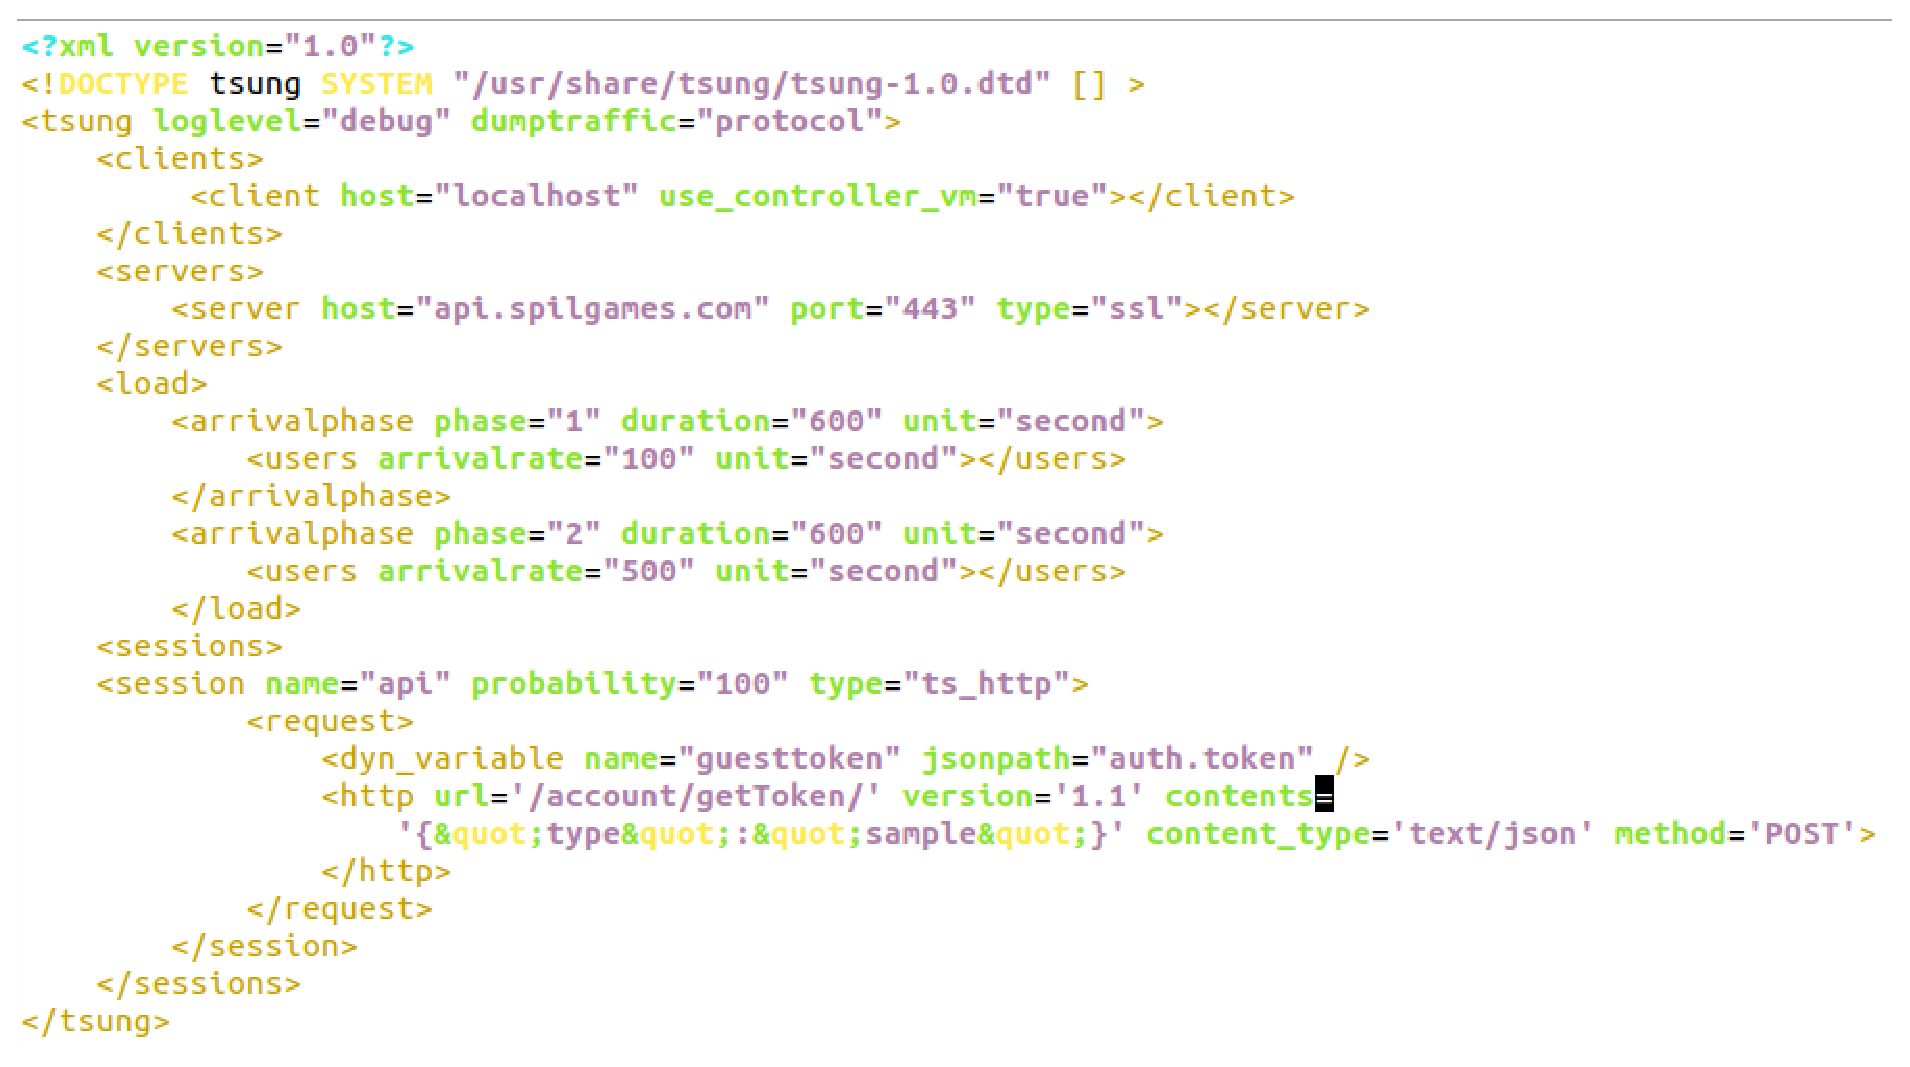
\includegraphics[scale=0.40]{images/tsung_spec.eps}
    \end{itemize}
\end{frame}

\begin{frame}{Basic Benchmarking}
    \begin{itemize}
    \item Testing a function doesn't have to be painful
    \pause
    \item The sooner you realize is bad, the less impact
    \pause
    \item \lstinputlisting{code/globalBenchmark.erl}
    \end{itemize}
\end{frame}

\begin{frame}{Basic Benchmarking}
    \framesubtitle{Sync Execution}
    \lstinputlisting{code/syncBenchmark.erl}
\end{frame}

\begin{frame}{Basic Benchmarking}
    \framesubtitle{Async Execution}
    \lstinputlisting{code/asyncBenchmark.erl}
\end{frame}

\section*{Making it happen}
\label{making_it_happen}

\subsection*{TDD (testing as soon as possible)}
\label{tdd}

    % Basic TDD idea
    % The purist TDD approach

\begin{frame}{The purist approach}
    \begin{enumerate}
    \item A developer receives some requirements from his manager, who ideally has writting some acceptance tests
    \pause
    \item He designs the simplest (flexible) solution fitting those requirements
    \pause
    \item He documents and specs the API, and implements only the exported functions headers all returning \emph{unimplemented}
    \pause
    \item He writes as many unit and integration tests as necesary for that API
    \pause
    \item He hands over his work to another developer, who after agreeing with the design fills the implementation until
    all the tests pass
    \end{enumerate}
\end{frame}

\begin{frame}{A more practical approach}
    \begin{itemize}
    \item Write the tests ASAP, if possible before writing the code itself
    \pause
    \item While implementing, keep in mind everything you write you have to test it
    \pause
    \item Start executing your tests ASAP, specially to validate those small simple functions you use all around (yes,
    those that \emph{can never fail})
    \end{itemize}
    \pause
    When changing exiting code
    \begin{itemize}
    \item Even if the existing coverage is poor, write tests for the changes you introduce
    \pause
    \item Make sure all the tests are running before touching a single line!
    \end{itemize}
\end{frame}

\begin{frame}{TDD refactor}
    \framesubtitle{Original Tests}
    \lstinputlisting{code/ageRefactor1.erl}
\end{frame}

\begin{frame}{TDD refactor}
    \framesubtitle{Original Code}
    \lstinputlisting{code/ageRefactor2.erl}
\end{frame}

\begin{frame}{TDD refactor}
    \framesubtitle{Updated Tests}
    \lstinputlisting{code/ageRefactor3.erl}
\end{frame}

\begin{frame}{TDD refactor}
    \framesubtitle{Updated Code}
    \lstinputlisting{code/ageRefactor4.erl}
\end{frame}

\subsection*{Automating everything}
\label{automating_everything}

\begin{frame}{CI Environment}
    \begin{itemize}
    \item Builds and tests a release your projects after every commit (Unit, Integration and Acceptance)
    \pause
    \item This automatic V\&V process should never take longer than 5 minutes
    \pause
    \item If the process fails, immediatly \emph{blames} the originator of the change
    \pause
    \item Long duration test suites can be put together in a regression task performed during the night
    \end{itemize}
    \pause
    \begin{equation*}
    \boxed{CI + AutomaticDeployment = ContinuousDelivery}
    \end{equation*}
\end{frame}

\begin{frame}{Keeping an eye on quality}
    \begin{itemize}
    \item Most CI systems have desktop or browser plugins
    \pause
    \item Screens on the wall can be an option as well
    \pause
    \item The quality of the final product starts with quality of your code
    \end{itemize}
\end{frame}

\begin{frame}{Measuring code quality}
    \begin{itemize}
    \item \emph{cover} can be integrated with eunit and Common Test to show you the test coverage
    \pause
    \item Dialyzer can detect typing errors and clear specs help a lot when testing
    \pause
    \item Open source tools such as Sonar analyse your code looking for risks
    \pause
    \item They point you to the weakest points of your source
    \pause
    \item Shows nice graphics about test coverage, unreachable code, nested code\dots
    \end{itemize}
\end{frame}

\begin{frame}{Quality control with Sonar}
\end{frame}

\section{Q\&A}
\subsection{}

\begin{frame}{Thanks Everyone!}
    \begin{itemize}
    \item Questions?
    \item Comments?
    \item Suggestions?
    \end{itemize}
\end{frame}
%
%% Everybody tests! (with clasical excuses)
%% Types of testing: unit, integration, acceptance, performance
%% Unit tests extended
%% Integration tests extended
%% Acceptance tests extended
%% Performance tests extended
%% How to make it painless: TDD (testing asap)
%    % Basic TDD idea
%    % The purist TDD approach
%% CI
%    % run tests &&  make doc && make release triggered on commit (blaming if necessary) [Jenkins]
%    % Deployed releases only come from succesful CI builds (even automatically!)
%    % CI info generation: coverae, static analysis... [Sonar]
%
%
%% Since this a solution template for a generic talk, very little can
%% be said about how it should be structured. However, the talk length
%% of between 15min and 45min and the theme suggest that you stick to
%% the following rules:  
%
%% - Exactly two or three sections (other than the summary).
%% - At *most* three subsections per section.
%% - Talk about 30s to 2min per frame. So there should be between about
%%   15 and 30 frames, all told.
%
%

\end{document}


